\documentclass{beamer}

\usepackage{polski}
\usepackage[utf8]{inputenc}
\usepackage{graphicx}
\graphicspath{ {/} }
\usepackage{listings}

\usetheme{CambridgeUS}
\usecolortheme{beaver}
\setbeamertemplate{section in toc}[sections numbered]
\setbeamertemplate{subsection in toc}[subsections numbered]
\setbeamercolor{section in toc}{fg=black}
\setbeamercolor{subsection in toc}{fg=gray}
\setbeamertemplate{enumerate item}[triangle]



\AtBeginSection[]
{
\begin{frame}<beamer>
% \frametitle{Spis treści}
\tableofcontents[currentsection]
\end{frame}
}


\title[Sieć neuronowa- rozpoznawanie cyfr]
{Algorytm sieci neuronowej}
\subtitle{Rozpoznawanie cyfr}
\author[Piotr Klimkowski  \and Rafał Borysionek]
{Piotr Klimkowski \and Rafał Borysionek}
\institute[]
{Wydział Elektroniki \\
Politechnika Wrocławska
}
\subject{Projektowanie Algorytmów i Metody Sztucznej Inteligencji}

\begin{document}


\begin{frame}
  \titlepage
\end{frame}


\begin{frame}
  \frametitle{Spis treści}
  \tableofcontents
\end{frame}

\section{Teoria Sieci Neuronowych}

\subsection{Baza danych MNIST}
\frame{
  MNIST czyli baza danych służąca do uczenia:
  \begin{figure}
  \centering
  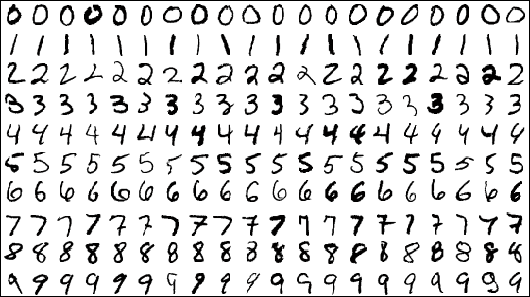
\includegraphics[height=4cm]{mnist.png}
  \end{figure}
}

\subsection{Architektura sieci}
\frame{
  \frametitle{Struktura sieci}
  \begin{figure}
  \centering
  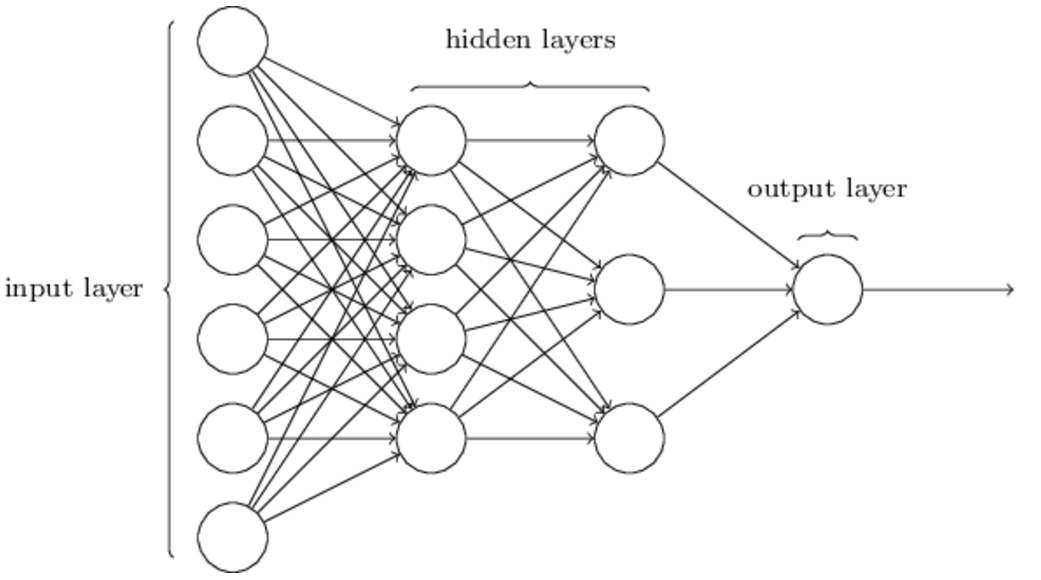
\includegraphics[height=4cm]{struktura.png}
  \end{figure}
}

\frame{
  \frametitle{Neuron w sieci}
  \begin{figure}
  \centering
  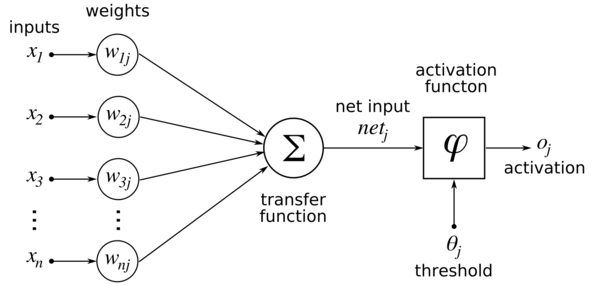
\includegraphics[height=4cm]{neuron.png}
  \end{figure}
}

\frame{
  \frametitle{Aktywacja neuronu}
  \begin{figure}
  \centering
  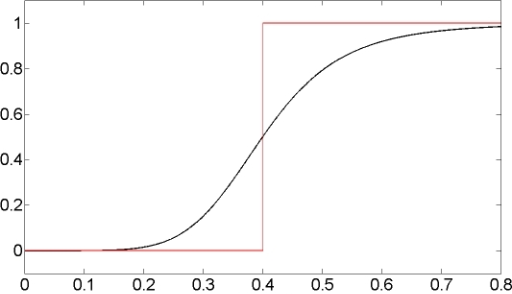
\includegraphics[height=4cm]{sigmoid.png}
  \end{figure}
}

\subsection{Metoda Gradientu}
\frame{
  \frametitle{Dopasowywanie wag}
  \begin{exampleblock}{Metoda najmniejszych kwadratów}
  \[
  Q=\sum(y-\hat{y})^{2}
  \]
\end{exampleblock}
}

\frame{
  \frametitle{Gradient}
  \begin{figure}
  \centering
  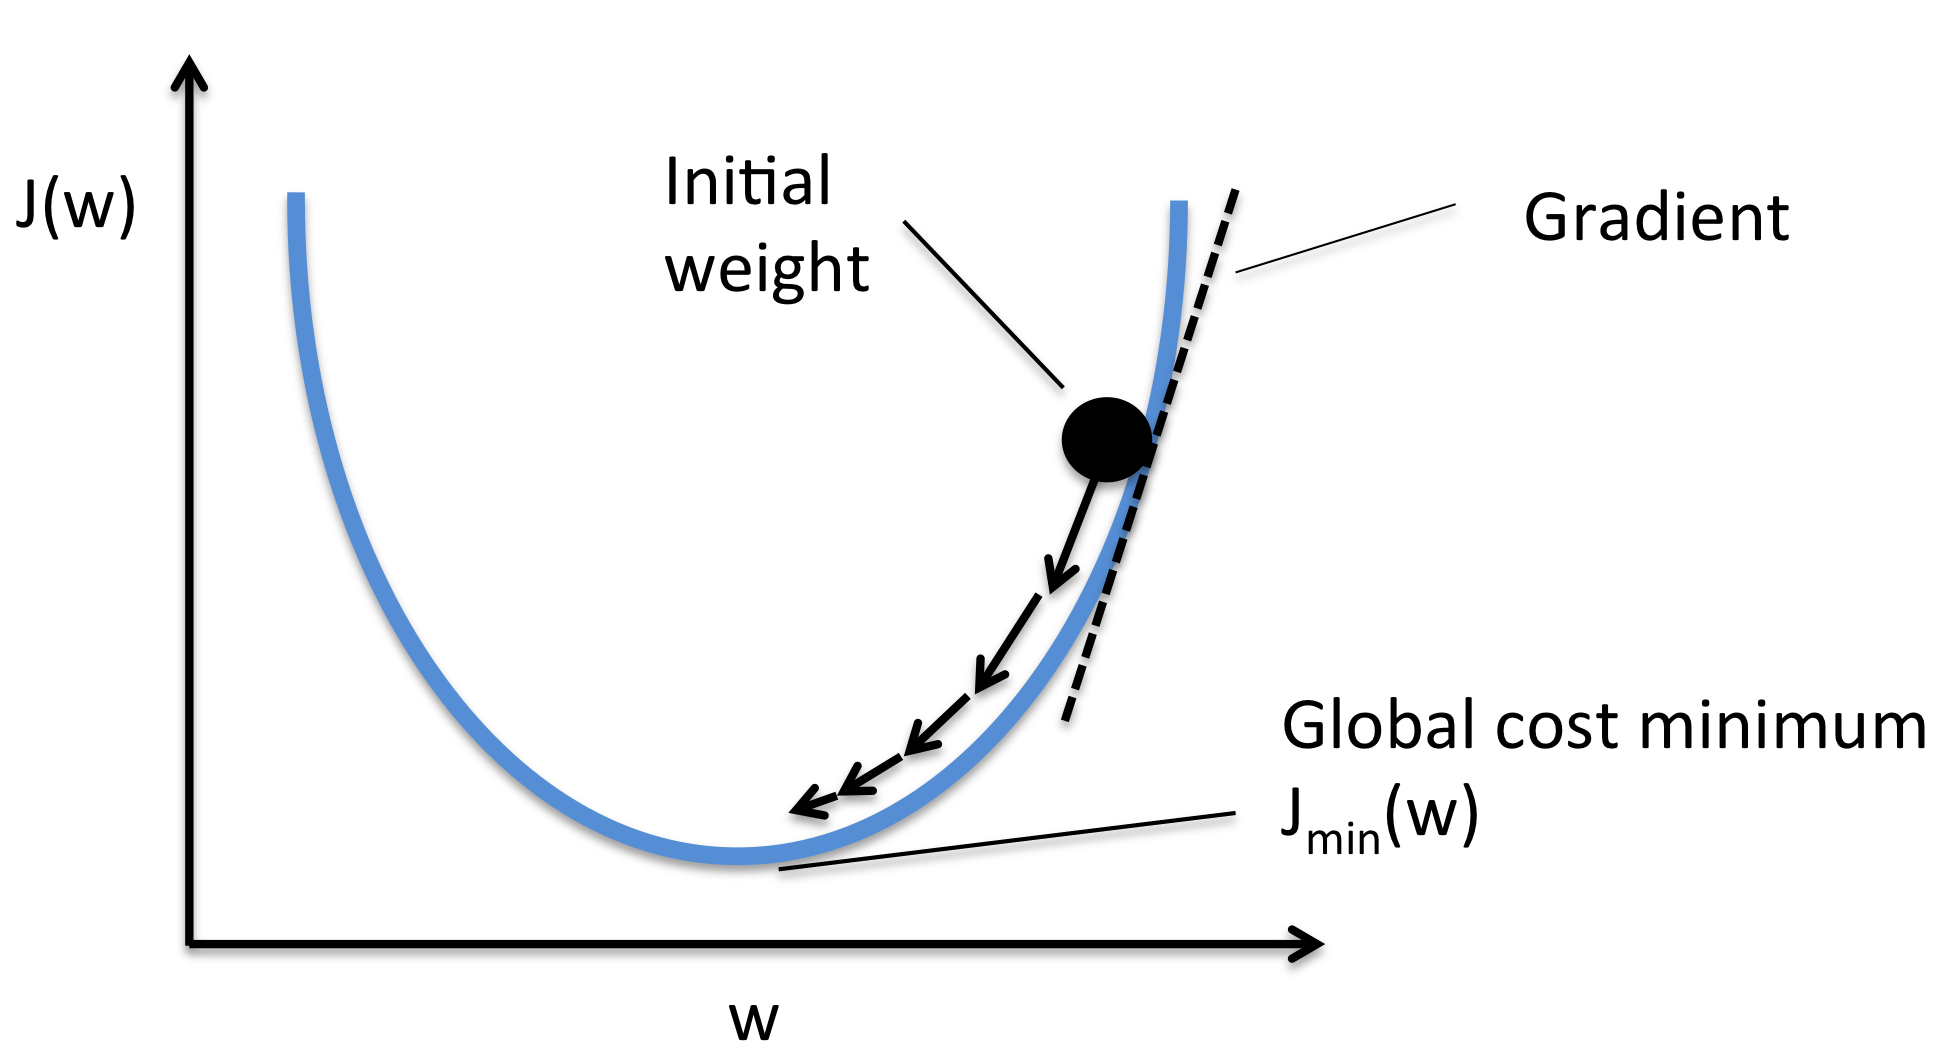
\includegraphics[height=4cm]{gradient.png}
  \end{figure}
}


\subsection{Backpropagation}
  \frametitle{Backpropagation}
  \frame{
  \begin{figure}
  \centering
  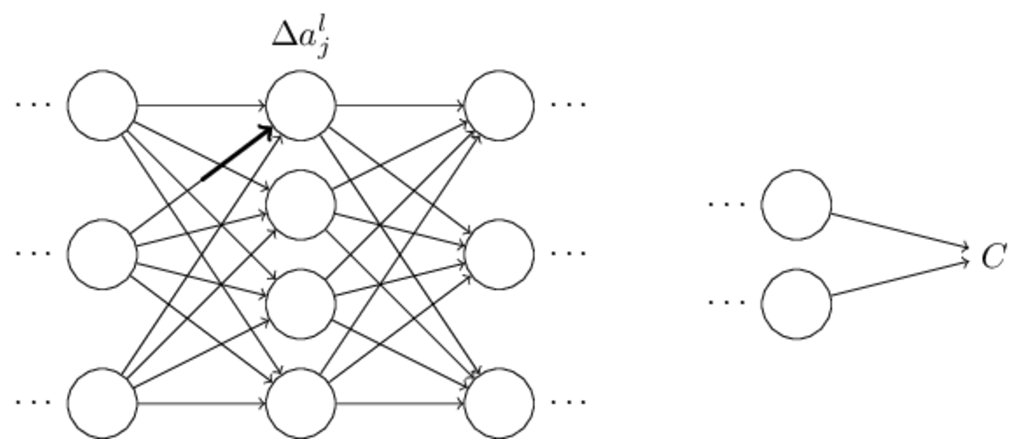
\includegraphics[height=4cm]{bak2.png}
  \end{figure}
}
\frame{
  \frametitle{Backpropagation}
  \begin{figure}
  \centering
  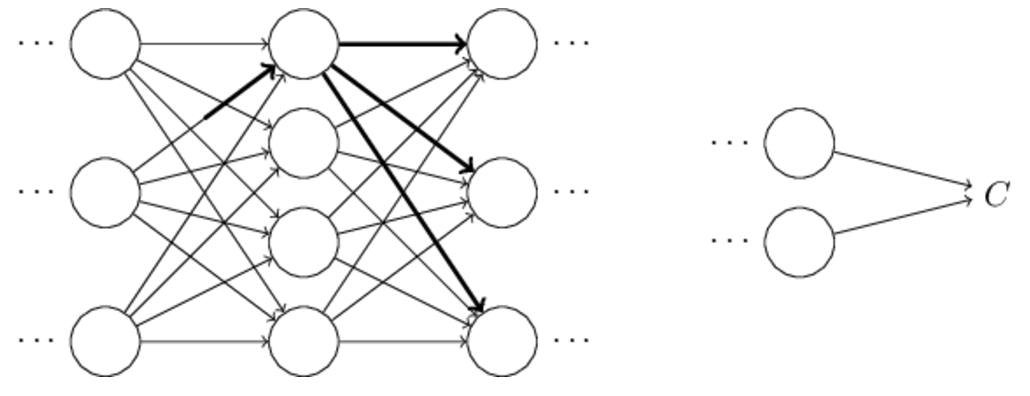
\includegraphics[height=4cm]{bak3.png}
  \end{figure}
}

\frame{
  \frametitle{Backpropagation}
  \begin{figure}
  \centering
  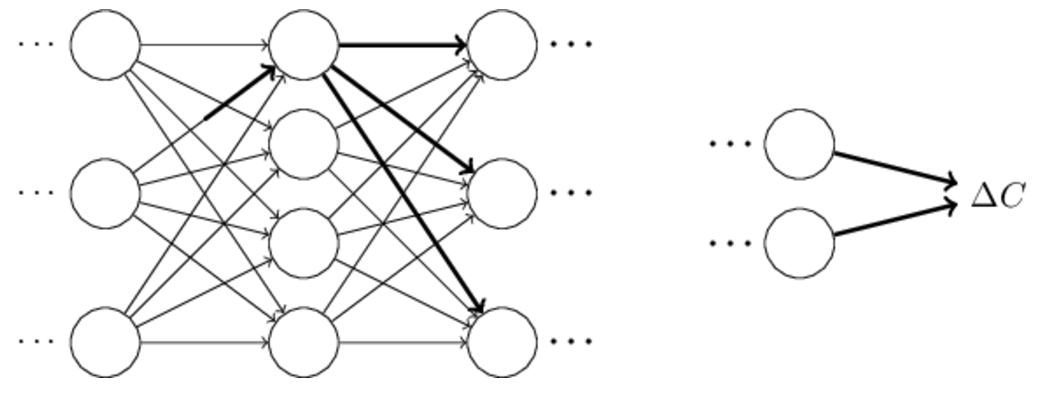
\includegraphics[height=4cm]{bak4.png}
  \end{figure}
}
\frame{
  \frametitle{Backpropagation}
  \begin{figure}
  \centering
  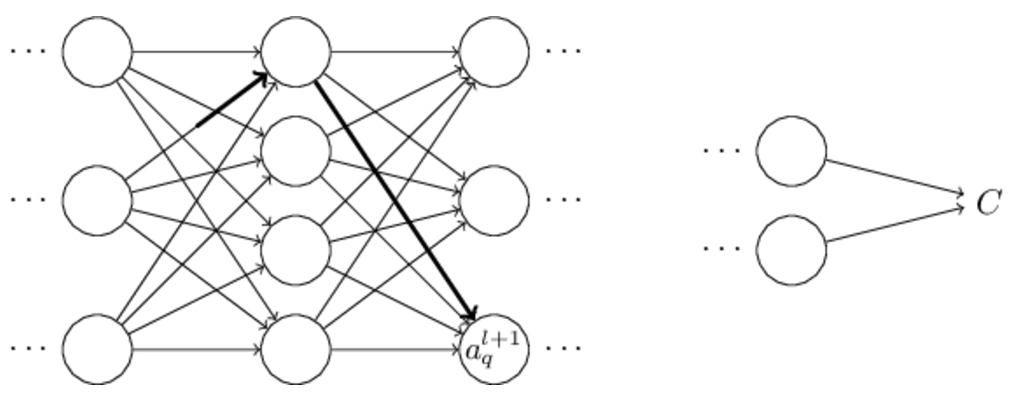
\includegraphics[height=4cm]{bak6.png}
  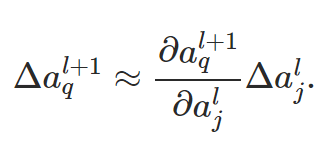
\includegraphics[height=1cm]{bak6_1.png}
  \end{figure}
}
\frame{
  \frametitle{Backpropagation}
  \begin{figure}
  \centering
  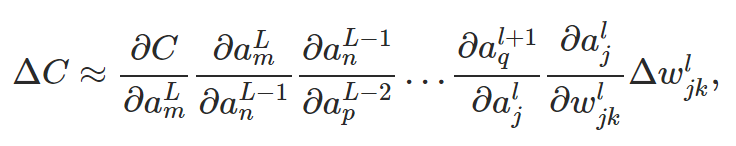
\includegraphics[height=2cm]{bak7.png}
  \end{figure}
}
\subsection{Overfitting}
\frame{
  \frametitle{Co to jest Overfitting?}
  \begin{figure}
    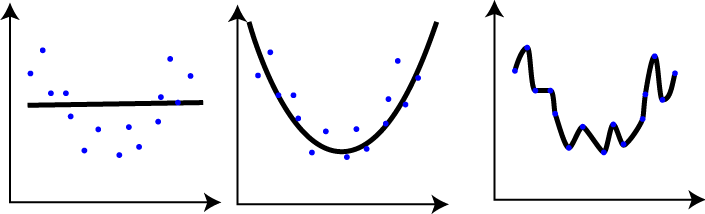
\includegraphics[scale=0.45]{coto.png}
  \end{figure}    
  }


\frame{
  \frametitle{Kiedy on występuje?}
  \begin{figure}
    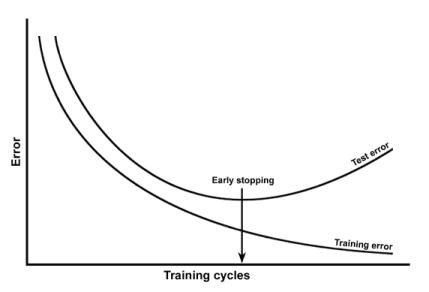
\includegraphics[scale=2]{kiedy.png}
  \end{figure}  
}
\subsection{Dropout}
\frame{
  \frametitle{Dropout jako sposób na overfitting}
  \begin{figure}
    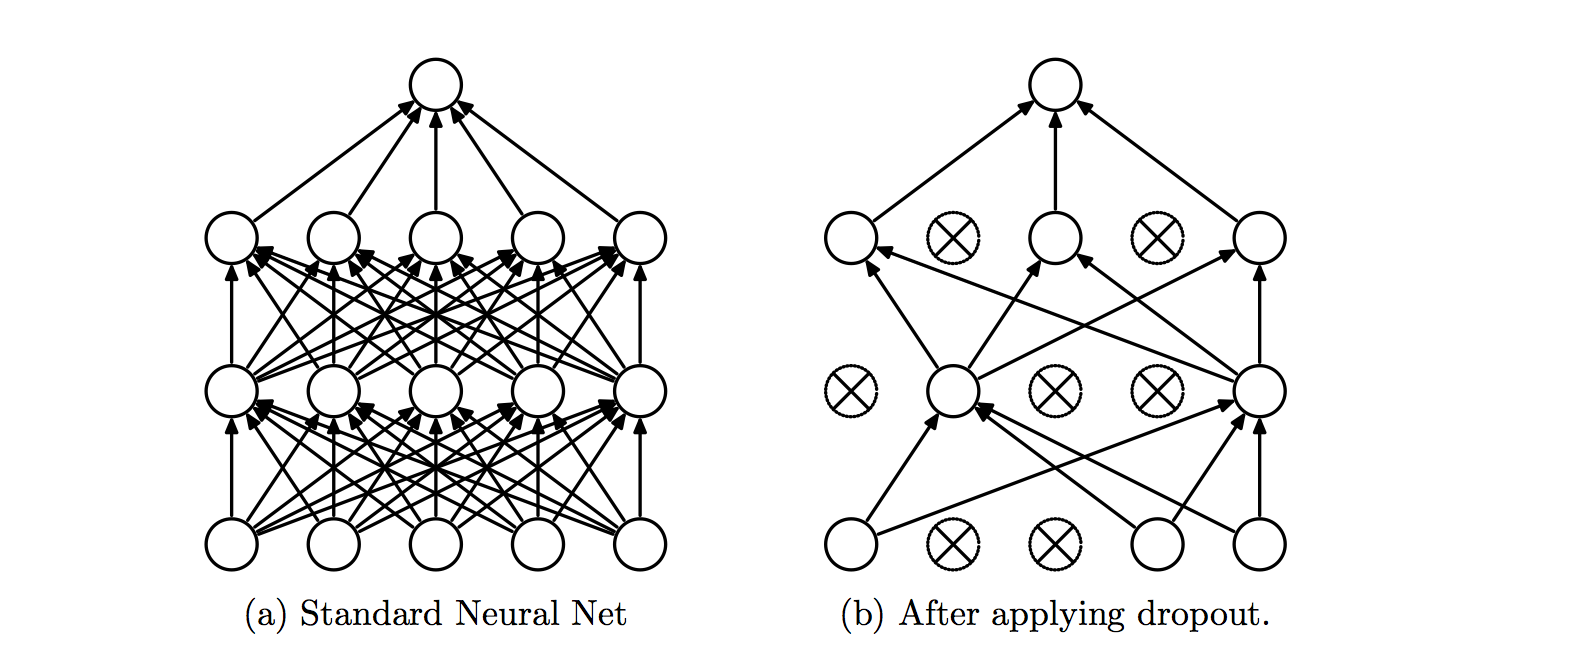
\includegraphics[scale=0.45]{drop.png}
  \end{figure}
}
\subsection{Konwolucje}
\section{Wyniki doświadczalne}
\subsection{Wpływ ilości ukrytych warstw na błąd}
\frame{
  \begin{table}
    \begin{tabular}{|l|r|}
      \hline
      \textbf{Warstwy} & \textbf{Błąd [\%]} \\
      \hline

800,400				&				2,32  \\
400,800				&				2,40\\
800				&    			2,41\\
400,400				&				2,42       \\
500,150				&				2,52\\
800,800		&	2,53\\
400,200,100		&				2,53\\
800,400,400		&				2,61\\
400,400,400			&				2,62\\
800,400,100		&				2,94\\
100,100,100			&				3,23\\

      \hline
      
    \end{tabular}
  \end{table}
    
}
\subsection{Wpływ ilości cykli uczenia na błąd}
\frame{
  \begin{figure}
    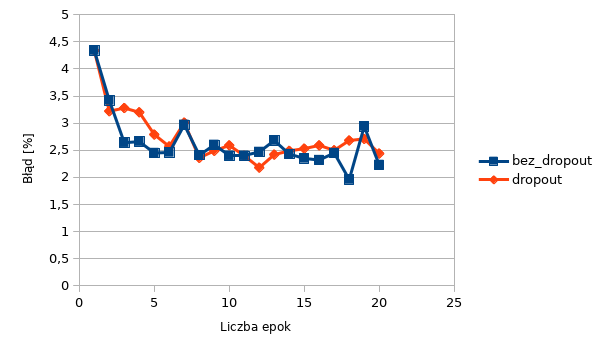
\includegraphics[scale=0.75]{wykres.png}
  \end{figure}
}
\section{Prezentacja programu}

\section{Bibliografia}
\begin{frame}[allowframebreaks]

 \frametitle{Bibliografia}
 \begin{thebibliography}{10}
 % \beamertemplatebookbibitems
 %powyzej wstawiamy ikonke ksiazki
 % \bibitem{Autor1990}
 % X.~Autor.
 % \newblock {\em Ei}.
 % \newblock Klein-Verlag, 1990.
 \beamertemplatearticlebibitems
 %powyzej wstawiamy ikonke ksiazki
 \bibitem{MNIST}
 Yann LeCun, Corinna Cortes, Christopher J.C. Burges.
 \newblock THE MNIST DATABASE of handwritten digits.
 \newblock {\em http://yann.lecun.com/exdb/mnist/}
 \beamertemplatearticlebibitems
 \bibitem{Github}
   Stephen Welch.
   \newblock Neural-Networks-Demystified.
   \newblock {\em https://github.com/stephencwelch}
   \beamertemplatearticlebibitems
 \bibitem{Keras}
   Keras Documentation
   \newblock Keras: The Python Deep Learning library.
   \newblock{\em https://keras.io/}
 
 \end{thebibliography}
 \end{frame}




\end{document}